\documentclass{article}
\usepackage{tikz}
\usetikzlibrary{arrows.meta}

\begin{document}

\begin{figure}[h]
    \centering
    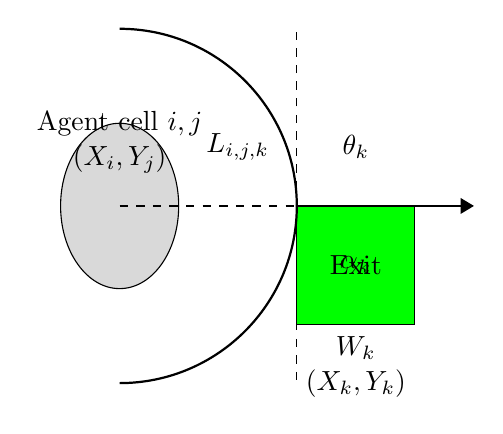
\begin{tikzpicture}[scale=1.5]
        
        % Exit sign
        \draw[fill=green] (0,0) rectangle (1,-1);
        \node at (0.5,-0.5) {Exit};
        \node at (0.5,-1.2) {$W_k$};
        \node at (0.5,-1.5) {$(X_k,Y_k)$};
        
        % Agent cell
        \draw[fill=gray!30] (-1.5,0) ellipse (0.5 and 0.7);
        \node at (-1.5,0.7) {Agent cell $i,j$};
        \node at (-1.5,0.4) {$(X_i,Y_j)$};
        
        % Lines and angles
        \draw[dashed] (-1.5,0) -- (0,0);
        \draw[dashed] (0,0) -- (1.5,0);
        \draw[dashed] (0,0) -- (0,1.5);
        \draw[dashed] (0,0) -- (0,-1.5);
        
        % Arcs
        \draw[thick] (0,0) arc (0:90:1.5);
        \draw[thick] (0,0) arc (0:-90:1.5);
        
        % Labels
        \node at (0.5,0.5) {$\theta_k$};
        \node at (0.5,-0.5) {$\alpha_k$};
        \node at (-0.5,0.5) {$L_{i,j,k}$};
        
        % Arrow
        \draw[-Triangle, thick] (0,0) -- (1.5,0);
        
    \end{tikzpicture}
    \caption{The projection surface of the exit sign being observed changes according to the viewing angle $\theta$. $\theta$ can be described as a function of the orientation of the sign in the global $z$-plane, expressed by the rotation angle $\alpha_k$, and the viewer's position at the agent cell $i,j$.}
    \label{fig:exit_sign_projection}
\end{figure}

\end{document}